\section{Frekvensgenerator}
I dette afsnit vil alle overvejelser omkring frekvensgeneratoren blive gennemgået, hertil designvalg og beregninger. 
\subsection{Design}
Til at genererer et signal ud fra batterierne anvendes en timer kreds. 
Timeren skal her bruges til at lave et puls signal der har en given frekvens og duty-cycle, dvs. et firkantet signal. 
Der er her valgt en konfiguration der hedder A-stabel. 
Fordelen ved dette er at timeren kan hente sit input direkte fra forsyning der i dette tilfælde er et batteri, dette koster en ekstra modstand men med den fordel at duty-cycle og frekvens bliver frie variabler. 
Dette signal skal have en frekvens der er tilpas høj så systemet er mindre modtagelig overfor forstyrrelse og det vil give en hurtigere respons. 

Timeren er designet til at lave et firkant signal, og det er også bestemt at dette signal sendes gennem spolen.
Skulle denne laves om til en sinus ville det kræve ekstra komponenter og lave en masse effekttab og give et langsommere system.

Signalet der kommer ud af timeren er begrænset således at udgangsspændingen kun kan antage positive værdier.
For at løse dette skal der sættes en kondensator i serie med spolen.
Dette gør at spolen bliver påtrykt en spænding af varierende polaritet, hvilket også giver et konstant skiftende magnetfelt.

\begin{figure}[h!]
	\centering
	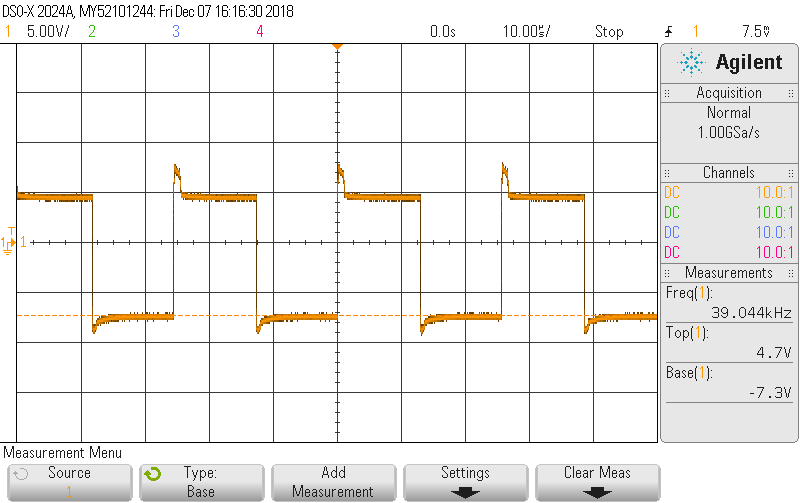
\includegraphics[width=1\textwidth]{billeder/freq_png.png}
	\caption{Her ses outputtet fra frekvensgeneratoren}
	\label{fig:frekvensgenerator}
\end{figure}

Inden kredsløbet tegnes færdigt skal der tages højde for den spænding timeren leverer. 
Spolen har en meget lille indre modstand, hvilket medfører at ved høje spændinger, skal timeren leverer en stor strøm. 
Da timeren ikke kan holde til at leverer mere end 225 \si{\milli\ampere}, sættes en modstand i serie for at begrænse strømmen. 
Det færdige kredsløb ses på figur \husk{Kenneth}{indsættelse af figur}

\subsection{Beregninger af komponenter}
Til udregning af modstand og kondensator værdier anvendes to af de ligninger der er opgivet i databladet for NE555 timeren. 
Først anvendes ligning 5 i data bladet til at bestemme modstanden $R_5$. 
Da der ikke er ligninger nok så bliver duty-cyclen og modstanden $R_6$ valgt. 
Duty-cyclen sættes til 51\%  , og $R_6$ vælges til 15 \si{\kilo\ohm}. 
Ligning 5 i databladet omskrives svarende til i ligning \ref{eq:TimerInputModstand}.
\begin{align}
R_5 & = \frac{R_6}{DutyCycle} - 2 \cdot R_6 \label{eq:TimerInputModstand}
\end{align}

Parametrene indsættes i ligning \ref{eq:TimerInputModstand}.
Resultatet viser her at $R_5$ skal være 588 \si{\ohm}  for at opnå en duty-cycle på 51 \% .
Som det sidste skal der udregnes en kondensator der forbindes til trigger indgangen og til ground. 
Til dette anvendes ligning 4 i databladet. Denne ligning isoleres for kondensatoren.
Modstandsværdierne er kendte, og der bestemmes her for en frekvens på $F_c = 50 \si{\kilo\hertz}$.
\begin{align}
	C_7 & = \frac{1}{F_c \cdot \left( \frac{25 \cdot R_5 }{36} + \frac{25 \cdot R_6}{18} \right) \label{eq:Kondensator_c7}}
\end{align}

Ud fra ligning \ref{eq:Kondensator_c7} fås en kondensator værdi $C_7 = 0.9\si{\nano\farad}$ for at få en frekvens på 50 \si{\kilo\hertz}. 
Da disse størrelser ikke kan realiseres i de lagerførte SMD værdier, vælges derfor tilnærmede værdier. 
Dette medfører at $R_5$ bliver 680 \si{\ohm} og $C_7$ på 1 \si{\nano\farad}. 
Heraf udregnes duty-cycle og frekvens ved at bruge ligning 4 og 5 i databladet.

I det praktiske kredsløb forventes der derfor en duty-cycle på 49 \% og en frekvens $F_c = 46.9 \si{\kilo\hertz}$. 
Duty-cyclen ligger tæt på 50 \% og frekvensen den ønskede frekvens er så stor at en lille afvigelse ikke kommer til at have en væsentlig betydning. Denne opstilling accepteres.

Der skal herefter sættes en kondensator på udgangen således at udgangsspændingen kan antage både positive og negative værdier. 
Middelspændingen over en spole er $0 \si{\volt}$, det er outputtet ikke, da den ikke oscillere omkring $0 \si{\volt}$, hvilket er kondensatorens formål. 
\subsection{Beregning af udgangskondensator}
For at kunne finde senderspolens impedans, anvendes vinkelfrekvensen $\omega_c$ som udregnes i ligning \ref{eq:vinkelfrekvens}.
\begin{align}
	\omega_c & = 2 \cdot \pi \cdot F_c \label{eq:vinkelfrekvens}
\end{align}
Der fås en vinkelfrekvens på $\omega_c = 294.910 \si{\kilo\radian\per\second}$.
Senderspolens induktans måles ved hjælp af en RLC-meter til $L = 205 \si{\micro \henry}$.
Det ønskes ikke at spolens impedans bliver lige så stor som kondensatorens, idet der så opstår en resonanskreds. 
Spolens impedans udregnes ved ligning \ref{eq:spole_impedans}
\begin{align}
	Z_L & = \omega_c \cdot L = 60.5 \si{\ohm} \label{eq:spole_impedans}
\end{align}
Der vælges her at spolens impedans skal være 20 gange større end kondensatorens impedans. Størrelsen på kondensatoren udregnes ved ligningen \ref{eq:kondensator_c9}.
\begin{align}
	Z_{C9} & = \frac{20}{\omega_c \cdot C_9} \rightarrow C_9 = 1.1 \si{\micro\farad} \label{eq:kondensator_c9}
\end{align}
Ved en kondensator størrelse på 1.1 \si{\micro\farad} er størrelsesforholdet mellem de 2 impedanser 20 gange. 
SMD kondensatoren der passer til er på 1 \si{\micro\farad}. Det praktiske størrelsesforhold udregnes igen hvor $C_9 = 1 \si{\micro\farad}$. Størrelsesforholdet bliver da $Z_L \cdot Z_c = 17.8$ gange, hvilket er acceptabelt.

På grund af modstanden og kondensatoren i kredsløbet, opstår der en forsinkelse i systemet, der er lig produktet af kondensatoren $C_9$ og modstanden $R_7$. $R_7$ er et potentiometer, så i beregningen anvendes højeste værdi, som er $1\si{\kilo\ohm}$.
\begin{align}
	\tau & = R \cdot C = 1 \si{\milli\second}
\end{align}
Forsinkelsen på $1 \si{\milli\second}$ er acceptabelt for systemet.

